\section{Decorators}


\subsection{Decorators}
\begin{frame}
\frametitle{Decorators}
	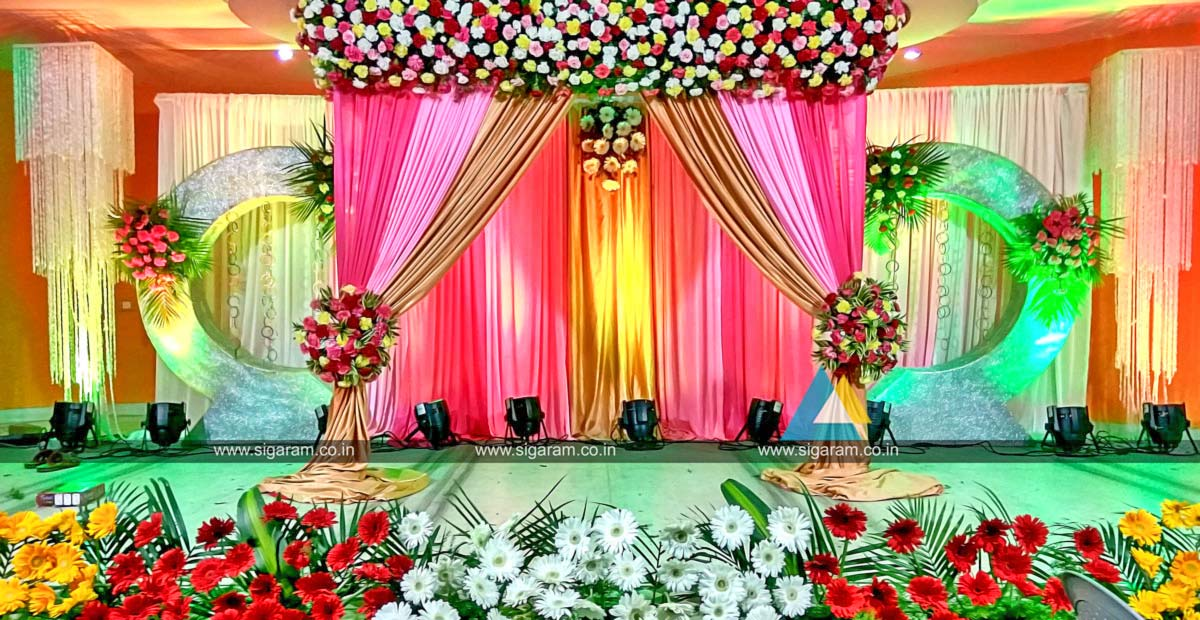
\includegraphics[width=0.9\textwidth]{img/decorators.jpg}
\end{frame}

\subsection{Decorators}
\begin{frame}
\frametitle{What is a Decorator}
\setlength{\epigraphwidth}{0.9\textwidth}
\epigraph{``A decorator is the name used for a software design pattern.
Decorators dynamically alter the functionality of a function, method, or class without having to directly use subclasses or change the source code of the function being decorated."}{--- https://wiki.python.org/moin/PythonDecorators}

\end{frame}

\subsection{Decorators}
\begin{frame}
\frametitle{What is a Decorator}
\setlength{\epigraphwidth}{0.9\textwidth}
\epigraph{``A decorator is the name used for a software design pattern.
Decorators dynamically alter the functionality of a function, method, or class without having to directly use subclasses or change the source code of the function being decorated."}{--- https://wiki.python.org/moin/PythonDecorators}

\end{frame}

\subsection{Decorators}
\begin{frame}
\frametitle{A simpler explanation}
Decorators help to write code that is easier to write and read.
It's so called "syntactic sugar".
\end{frame}

\subsection{Decorators}
\begin{frame}
\frametitle{Example}
Decorators help to write code that is easier to write and read.
It's so called "syntactic sugar".
\end{frame}




%
%\subsection{Introduction}
%\begin{frame}[fragile]
%\frametitle{Bonus: Map Tools}
%\begin{lstlisting}[style=pythoncode]
%def onCanvasClicked(self, point, mouseButton):
%    """Calculate the average floor numbers over a 20x20 map units (meters for Switzerland) area"""
%    request = QgsFeatureRequest()
%    request.setFilterRect(QgsRectangle(point.x()-10, point.y()-10, point.x()+10, point.y()+10))
%    features = self.buildingsLayer.getFeatures(request)
%    
%    floors = [feature['floors'] for feature in features]
%    
%    avg = sum(floors)/float(len(floors))
%    print('Average floor number in this region is {}'.format(avg))
%
%mapTool = QgsMapToolEmitPoint(iface.mapCanvas())
%mapTool.canvasClicked.connect(self.onCanvasClicked)
%iface.mapCanvas().setMapTool(mapTool)
%\end{lstlisting}
%
%\subsection{What they are}
%\begin{frame}
%\frametitle{You know}
%\begin{itemize}
%	\item @qgsfunction
%	\item @alg
%	\item \_\_repr\_\_
%	
%\end{itemize}
%\end{frame}